\documentclass{article}
\usepackage[utf8]{inputenc}
\usepackage[T1]{fontenc}

\title{Rapport Apprentissage Automatique}
\author{Gabin Marc Mberi-Kongo, Quentin Vigne, Vincent Deschaud}
\author{Thomas Cambon, Florent Jakubowski }
\author{
  Gabin Marc Mberi-Kongo\\
  \texttt{gabin.mberi-kongo@univ-lyon2.fr}
  \and
  Quentin Vigne\\
  \texttt{quentin.vigne@univ-lyon2.fr}
  \and
  Vincent Dechaud\\
  \texttt{vincent.dechaud@univ-lyon2.fr}
  \and
  Thomas Cambon\\
  \texttt{t.cambon@univ-lyon2.fr}
  \and
  Florent Jakubowski\\
  \texttt{florent.jakubowski@univ-lyon2.fr}
}
\date{February 2021}

\usepackage{natbib}
\usepackage{graphicx}

\begin{document}

\maketitle

\tableofcontents

\section{Introduction}

Dans le cadre du module Apprentissage supervisé dispensé par Monsieur Ah-pine, nous avons eu le choix d'implémenter un algorithme d'apprentissage supervisé parmi plusieurs et de tester ses performances par rapport à d'autres méthodes d'apprentissage supervisé. 

\section{Sujet}
Nous avons choisis parmis les 4 sujets proposés le sujet sur l'algorithme Adaboost.
\section{Problématiques scientifiques}
La problématique scientifique pour ce projet est de vérifier l'intérêt des méthodes dites d'ensembles pour la classification binaire et multiclasses. L'enjeux sera d'observer la différence de performance entre des méthodes d'apprentissage supervisé ne se basant pas sur une prédiction par comité et des méthodes qui au contraire utilisent le vote par comité pour faire leur prédiction.
Nous sommes appuyés sur l'implémentation de l'algorithme adaboost et de sa variante l'algorithme Adaboost M1 telle que décrite dans le 'papier' de Freund et Schapire \citep{FreundSchapire1996} en 1996 pour reimplémenter nos algorithmes.

\section{implémentation}
Pour l'implémentation nous avons chosis une approche par classe.

\section{Présentation du jeu de données}

Pour ce projet, nous avons choisi d'utiliser un jeu de données avec différentes informations sur des projets Kickstarter de 2018. Kickstarter est une entreprise de financement participatif qui donne la possibilité aux internautes de financer des projets qui n'ont pas encore été développés.\newline 

\noindent Le fichier csv que nous avons utilisé contient les variables suivantes : \newline 
\begin{itemize}
    \item ID du projet (ID)
    \item Nom du projet (NAME)
    \item Catégorie principale (MAIN\_CATEGORY)
    \item Sous-catégorie (CATEGORY)
    \item Monnaie utilisée (CURRENCY)
    \item Date limite pour le financement participatif (DEADLINE)
    \item Somme d'argent (GOAL) que souhaite récolter un créateur pour financer son projet (si la somme n'est pas atteinte, le projet ne sera pas financé et le créateur ne recevra pas d'argent)
    \item Date de lancement du projet (LAUNCHED)
    \item Montant total promis par les contributeurs pour le projet (PLEGED)
    \item Nombre de contributeurs (BACKERS)
    \item Pays (COUNTRY)
    \item Conversion en USD (USD\_PLEGED) du montant total promis par les contributeurs pour le projet (conversion effectuée par kickstarter) 
    \item Conversion en USD (USD\_PLEGED\_REAL) du montant total promis par les contributeurs pour le projet (conversion depuis l'API Fixer.io)
    \item Et enfin la somme d'argent que souhaite récolter un créateur pour financer son projet, convertie en USD (USD\_GOAL\_REAL).\newline 

\end{itemize}

\noindent La variable que l'on essayera de prédire est l'état du projet (STATE). Six états sont possibles :

\begin{itemize}
    \item Projet réussi (successfull)
    \item Projet échoué (failed)
    \item Projet en cours (live)
    \item Projet annulé (canceled)
    \item Projet suspendu (suspended)
    \item Ou projet non défini (undefined).\newline 
\end{itemize}

\noindent Voici un extrait des données :

\begin{center} 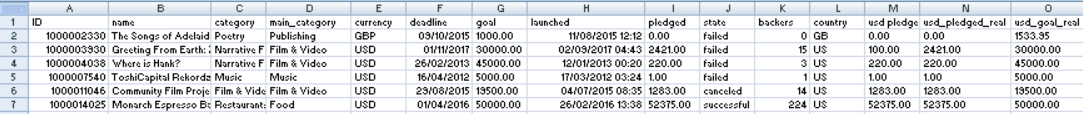
\includegraphics[scale=0.55]{extrait_donnees.PNG} \end{center}
\noindent Ce jeu de données est intéressant car il a un nombre important d'individus et de variables. De plus, il possède à la fois des variables catégorielles et numériques, ce qui donne de la variété dans les types de variables. \newline

\noindent Pour la suite, nous avons décidé de supprimer les colonnes ID et NAME car ce sont deux variables qui ont des valeurs uniques pour chacun des projets. Nous avons également supprimé les variables GOAL, PLEGED et USD\_PLEGED pour ne garder qu'une unique version de ces variables avec la devise USD.\newline

\noindent Nous conserverons uniquement les projets à l'état "successful" ou "failed" pour l'algorithme adaboost binaire. "Successful" prendra la valeur 1 et "failed" la valeur 0.\newline

\noindent Pour l'extension adaboost.M1 (problèmes multiclasses), nous garderons cette fois-ci tous les individus.


\section{le protocole expérimental}
Pour le protocole expérimental nous avons choisis plusieurs autres algorithmes d'apprentissage supervisé n'utilisant pas le vote par comité. 

Pour la classification binaire nous avons choisis les algorithmes suivant : 
Pour la classification multiclasse nous avons choisis les algorithmes suivant : 

Nous avons entrainé nos 2 algorithmes et les autres algorithmes avec le même nombre d'époques et le même data set. 
Puis nous avons comparé leurs prédictions avec les prédictions des autres algorithmes choisis à l'aide d'une fonction d'erreur.

La fonction d'erreur calcule le pourcentage de mauvaises prédictions données sur les données de test. 

\section{les résultats expérimentaux et leurs analyses}
Tableau des résultats exprimentaux obtenus

\section{une discussion scientifique/analyse critique}

\section{Conclusion}
Ici c'est la conclusion 
C'est terminé

\bibliographystyle{plain}
\bibliography{references}
\end{document}
